%!TEX root = ../thesis.tex
\chapter{Conclusions and Future~Work}
\label{chap:conclusion}

On the one hand there remain many unknowns about the explosions and progenitors of \sneia. On the other hand, there are many question that have been answered. The community has the unified believe that the \snia\ phenomenon is caused by the explosive burning in degenerate carbon and oxygen material. This suggests with a high probability a \gls{cowd} - a remnant of a 0.5~\msun\ to 8~\msun star. Traditionally there have been two assumptions: first that a \gls{cowd} will accrete from a \gls{mainsequence} to \gls{redgiant} companion - known as the \gls{sds}; second that this growth will end at the \gls{mchan} and the \gls{cowd} will explode as a \snia. 

Recent work by several authors \citep[e.g.][]{2011arXiv1106.4008B, 2010ApJ...722.1691H, 2010MNRAS.407.1314M} has started to suggest that at least one of these assumptions - the \gls{sds} - is unlikely to be entirely responsible for the bulk of \sneia. These authors often suggest the merger of two white dwarfs - known as the \gls{dds} - as the favoured scenario. Accreting mass to achieve 1.38\,\msun\ is one of the difficulties, especially in the \gls{sds}, which led some authors to speculate on a lower explosion mass of 1 -- 1.2\,\msun \citep[e.g.][]{2010ApJ...714L..52S} where stars explode, rather than reaching the \gls{mchan}, via a detonation on the stars' surface which triggers a detonation in the stars' center. 

This thesis is trying to address both the question of the progenitor as well as the explosion mass. The \gls{sds} predicts that post-explosion the companion star of a \snia\ is easily visible. In this thesis we have tried to find these companion stars, but to no avail in the two most favourable cases. 
Secondly to address, among other questions, the progenitor mass we have started to automate the fitting of \snia\ spectra. This technique has been applied successfully to a handful of supernovae \citep{2007Sci...315..825M}, but is currently only possible manually. The automation is technically very challenging, but we have currently completed two milestones - the ability to calculate many solutions in a cloud-like environment and the implementation of \glspl{ga} as the optimization algorithm of choice. 

This thesis has contributed important pieces of the puzzle that is the \snia\ phenomenon, but the question remains: How and why do these objects explode?

\section{Single or Double Degenerate?}
\glsreset{aic}
\glsreset{rlof}
The initial idea for this thesis was simple: High resolution spectroscopy and high precision astrometry of close and young \snia\ remnants should reveal the suggested donor star. At this time the only viable scenario was the \gls{sds}. The \glspl{dds} were almost unanimously believed to lead to \gls{aic} and not \sneia. The first project (Chapter \ref{chap:sn1572_starg}) was to confirm \starg\ as the progenitor of \sn{1572}{} and then move on and find the progenitors in both \sn{1006}{} and \sn{1604}{}.

The observations however started to show a completely different picture. The very unusual kinematics claimed for \starg\  by \citet{2004Natur.431.1069R}, were only slightly unusual. Comparison with the Besan\c{c}on Galactic model suggested the unusual radial velocity to actually be typical if \starg\ was placed at a distance that would make it compatible with a background interloper (see Section \vref{sec:sn1572:interloper}). This problem plagues kinematic evidence, and it motivated us to find a more tangible feature. The \gls{sds} in almost any viable scenario has \gls{rlof} as the means of mass transfer. A consequence of this mass transfer mode is tidal coupling of the donor star's rotation to the orbital rotation. This tidal coupling also implies that the rotation of the donor post-explosion is coupled to its escape velocity (see Section \vref{sec:sn1572_starg_rot} and Figure \vref{fig:theorot}). Most low-mass stars (spectral type later than F) rotate much less than the predicted rotational velocity of a donor post-explosion - leading to a powerful new diagnostic for donor stars. Our work in Chapter \ref{chap:sn1572_starg} indicated that \starg\ does not have an unusually high rotation. Follow-up work with improved data (see Chapter \ref{chap:sn1572_hires}) established this low rotation not only for \starg\ but also for five other stars close the the centre of \sn{1572}. While this finding is not entirely without caveats, as the rotation might vanish post-explosion if the star sufficiently increases its radius. In addition, the observable is not the rotation but the projected rotation ($\vrot\sin{i}$). However, if $\sin{i}$ would approach zero we would expect the star to have a high proper motion in the plane of the sky (because the rotation and orbit will be in the same plane). None of our candidates show such a trait (see Figure \vref{fig:propmot_sn1572_hires}). 
We have, however, found one star that exhibits very high rotation (consistent with the predictions for a donor star). However, this star (\starb) is a hot A-star where high rotation is not unexpected. In addition, we found \starb\ to have a very low spatial velocity. As the escape velocity and the rotational velocity are coupled we would expect a high spatial velocity for such a high rotation. Finally, we have calculated a distance from measurements of the surface gravity and temperature, which suggests \starb\ to be a foreground star. We conclude that observations of the stars in the remnant of \sn{1572}{} strongly suggest that \sn{1572}{} has no surviving \gls*{donor} star. 

Finally, for \sn{1572}{}\ we have found one more central bright star that thus far has eluded spectroscopic scrutiny. This star (Tycho-A2 by our nomenclature) has an unusual proper motion (see Figure \vref{fig:propmot_sn1572_hires}) and is located very close to the \xray\ center of \sn{1572}{} making it a prime candidate. Unfortunately Tycho-A2 hides 0.4\arcsec away from the 4 magnitude brighter \stara\ (see Figure \ref{fig:stara2_overview}), making it impossible to obtain ground-based optical spectroscopy, but offers the possibility for challenging infrared observations aided by adaptive-optics. We are currently running a \gls{gnirs} campaign to obtain the fundamental stellar parameters, radial velocity and rotation.  Initial measurements indicate this star does not possess unusual characteristics, and may be very similar to \stara.

\begin{figure}[tb] %  figure placement: here, top, bottom, or page
   \centering
   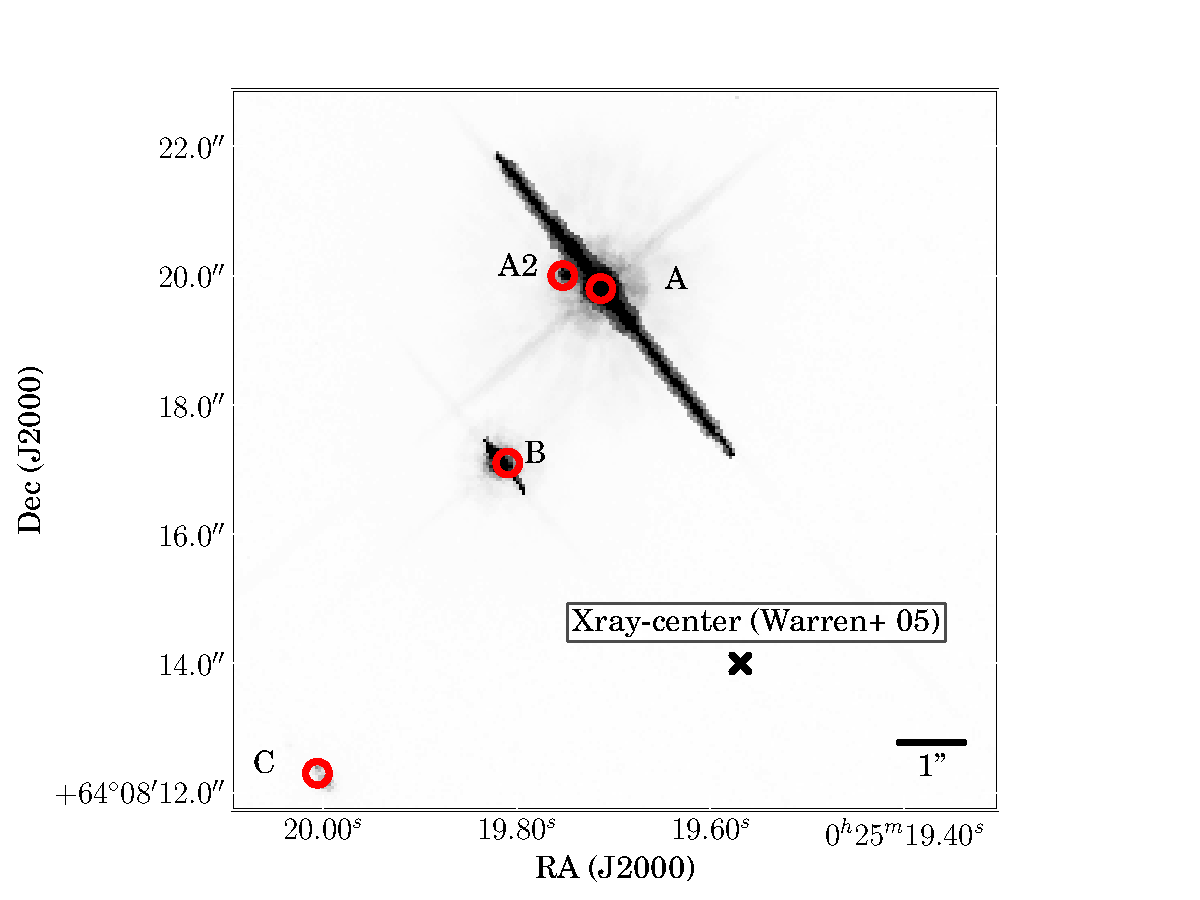
\includegraphics[width=\textwidth, trim=0 0 2cm 0, clip]{chapter_conclusion/plots/overview_sn1572_a2.pdf} 
   \caption[Close-up of the inner region of SN 1572 with candidates]{Overview of inner region of the remnant of SN1572. All labelled stars except Star-A2 have existing high-resolution spectra. Tycho-A2 is located very close to Tycho-A (0.6\arcsec). Spectroscopy can only be obtained with adaptive optics in the infrared.}
   \label{fig:stara2_overview}
\end{figure}

The second remnant we scrutinised was \sn{1006}{} (see Chapter \ref{chap:sn1006}). Using the \gls{flames} instrument on the \gls{vlt} we obtained spectra of stars around the centre to a limiting magnitude of $V<19$. Our primary set were stars with $V<17.5$, resulting in complete coverage of all stars with $L(V) > 0.5\lsun(V)$ at the distance of the remnant. Models predict any remaining \gls*{donor} star with much higher luminosity \cite[10--100\lsun][]{2000ApJS..128..615M}, although a range of luminosities are possible \citep{2003astro.ph..3660P}. 
We have analysed our prime candidate list for \vrot, \gls{teff}, \gls{feh} and \gls{logg} and again find no stars to have unusual rotation or spatial velocity. Stars fainter than $L < 0.5~\lsun$ have not all had their parameters extracted due to their low \snratio, although we have identified a path to estimate these quantities from the data in hand. However, models of single degenerate progenitors due not predict donor stars of such low luminosity. These results are consistent with our finding for \sn{1572}{} - no identifiable \gls*{donor} star. 

The bottom line for both \sn{1572}{} and \sn{1006}{} seems to be that there are no remaining donor stars as predicted by the \gls{sds}'s models. If \snia\ \gls*{donor} stars exists, they must be much different than predicted by models. Although there are always caveats, we do not think that with current theoretical knowledge and instrumentation it is worthwhile to scrutinise candidate stars in either remnant further. One exception might be the use of multi-epoch photometrically deep observations of these remnants to look for a hot white dwarf or helium star, not detectable by our current data, suggested by some new models \citep[e.g.][]{2010A&A...514A..53F}. 

\section{The curious case of Kepler}
\glsreset{csi}
The last of the young, moderately extinguished Galactic remnants, and the most distant one \citep[][estimates a distance of $\ge 6$\,\kpc]{2008ApJ...689..231V}, is \sn{1604}{} - also known as Kepler's supernova.  The morphology of this remnant is not as clean and spherical as \sn{1006}{}\ and \sn{1572}{}\ (see Figure \ref{fig:sn1604_observations}). For a long time \sn{1604}{}\ was believed to be a \snib, but prominent iron emission in \xray\ spectra \citep{2007ApJ...668L.135R} suggests this event to be a \snia\ \citep{1995ApJ...444L..81H}. \sn{1604}{} shows an abundance in nitrogen which is unusual for a \snia, and shows evidence for \gls{csi}. In addition, \citet{1991ApJ...366..484B} and \citet{2003A&A...407..249S} find that the remnant itself possesses a very high systemic velocity of  $\approx 250\,\kms$. A recent study by \citet{2011arXiv1103.5487C} suggests that a \gls{sds} with an \gls{agb} star as a \gls*{donor} would explain all of the observed peculiarities. In addition, \citet{2011arXiv1103.5487C} make the prediction that this star should be visible and very bright post-explosion. 

\begin{figure}[tb] %  figure placement: here, top, bottom, or page
   \centering
   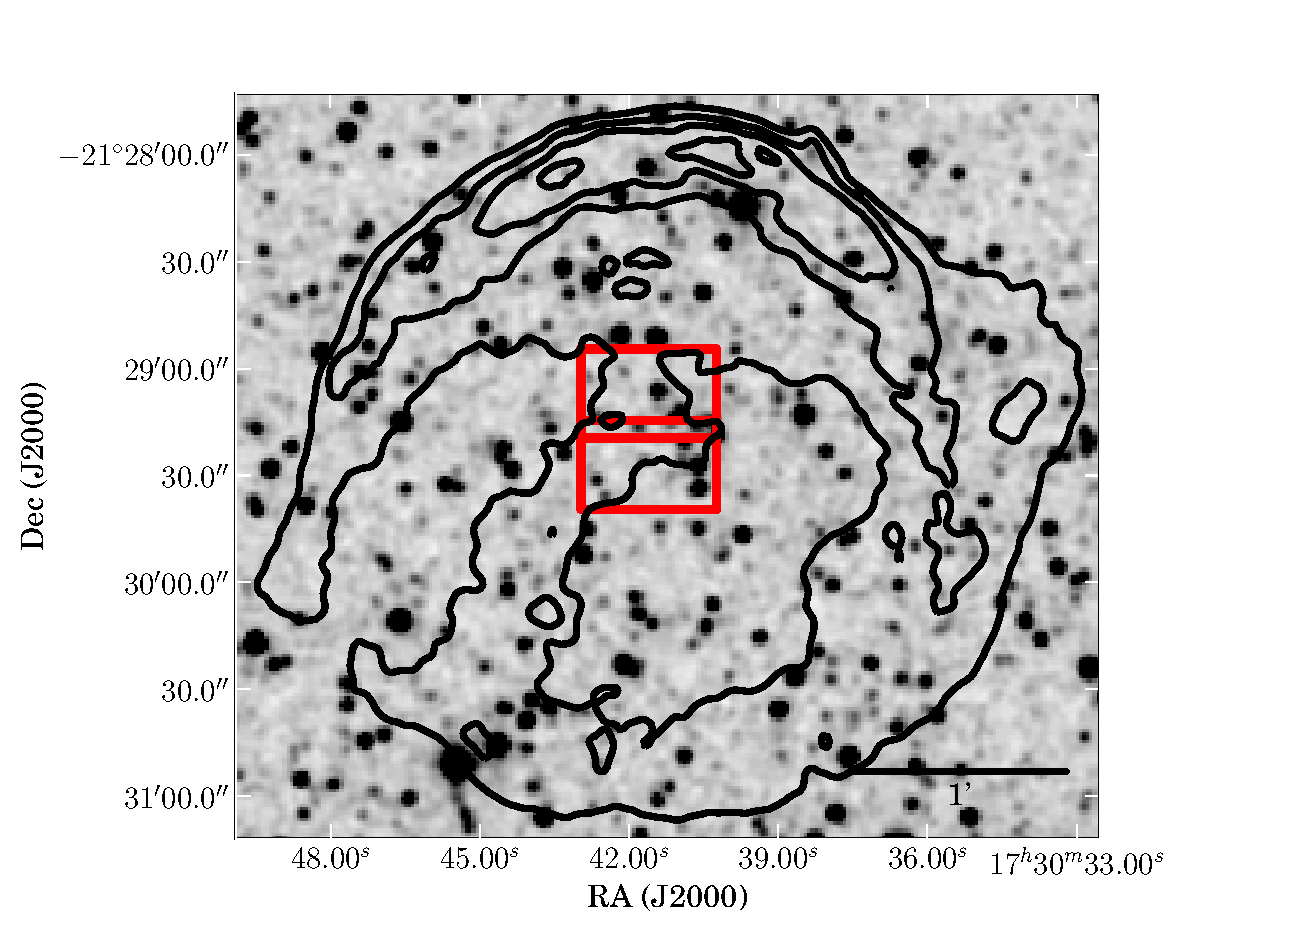
\includegraphics[width=\textwidth, trim=0 0 2cm 0, clip]{chapter_conclusion/plots/sn1604_overlay.pdf} 
   \caption[VLA contours of Kepler's remnant (SN1604) overlayed on a 2MASS image]{VLA contours of Kepler's remnant (SN1604) overlayed on a \twomass\ image. The red rectangle show the overlapping north and south field of our WiFeS observing campaign.}
   \label{fig:sn1604_observations}
\end{figure}

We have obtained data with the \gls{wifes} integral field spectrograph of \sn{1604}{}. The field of view for this instrument is rectangular with dimensions of $25\arcsec \times 38\arcsec$, sampled at 1.1\arcsec. We have two overlapping fields that cover all stars at a projected velocity of 1300\,\kms (assuming a distance of 6\,\kpc) (see Figure \ref{fig:sn1604_observations}). Extracting stellar spectra from our poor seeing data ($> 1.5\arcsec$) is technically challenging and we have not yet attempted this work.

A very recent study \citep{2011arXiv1108.1207W} has suggested that a fourth \snia\ remnant has features that suggest a \gls{sds}. This remnant - \gls{rcw86} - shows large amounts of iron in the \xray\ spectrum and no central neutron star has been found potentially indicating a \snia\ event. A distance of 2.5\,\kpc\ places it between \sn{1006}{} and \sn{1572}{} a territory that we are very familiar with. We plan to observe this remnant, like \sn{1006}{}\ with \gls{flames} in the coming semester.



\section{Divide et impera}

Maybe finding the progenitors of \sneia\ is too difficult using our current techniques. It might be much easier to employ the successful ``Divide et Impera'' - ``Divide and Conquer'' strategy. We believe it might be sensible to divide the question of the progenitor into accretion method and the mass of the \gls{cowd} at the time of explosion. For the accretion method in the \gls{sds} tests seem to frequently fail (e.g. no donor in remnants, not enough \glspl{sss}) and for the \gls{dds} there are no strong testable predictions yet. We believe a different path - namely understanding the explosion mechanism (delayed detonation or pure detonation) and \gls{cowd} mass at explosion might be the best way forward.  In terms of explosion mass there are currently two favoured scenarios. First the explosion of a \gls{cowd} close to \gls{mchan} (1.38\,\msun). As shown in Chapter~\ref{chap:intro} the burning of a 1.38\,\msun\ \gls{cowd} only produces the right abundance pattern when introducing a (slightly contrived) delayed detonation. When exploding a 1\,\msun\ \gls{cowd} this problem does not exist, a detonation of such a star produces the right optical photospheric spectrum \citep{2010ApJ...714L..52S}. The main problem with these sub \gls{mchan} explosions is that there exists no incontrovertable theory for the ignition yet - however some suggestions exist \citep[e.g.][]{2010A&A...514A..53F}. 
We believe that fitting many \snia\ spectra in the photospheric phase might yield the answer to the explosion mechanism and might help differentiate between viable explosion mechanisms through abundance patterns and mass estimates. We are currently exploring this option with the \gls{dalek}.
Another key to find the explosion mass of any given \snia\ might be the abundance of stable iron in nebular spectra. Theory predicts more iron for the \gls{mchan} case and less for the  sub \gls{mchan} scenario, and that the sub \gls{mchan} case should produce far less stable iron group elements.

\section{The Dalek Code}

We have presented two major milestone of the automatic fitting process of \sneia\ (see Chapter \ref{chap:dalek}). For the actual synthesis of the spectra we have chosen the \gls{mlc} code as it strikes the right balance between speed and accurate representation of the spectra for this task. 
In a first step we have wrapped the \gls{mlc} and enabled it to access a cloud-like computing environment (heterogeneous computing environment). This makes it very easy to test different optimization algorithms in a speedy and efficient manner. As the parameter space for \snia\ fitting is extremely complex and large, the automation is a technically challenging and ambitious project. We have however shown that \glspl{ga} are able to solve this problem. To continue our advancement of this problem, we have added two \gls{ga} experts to our team, which initially consisted only of radiative transfer experts and observers. Currently we are fine-tuning our \glspl{ga} with our newfound skill base and will soon try to fit many \snia\ spectra. Similar to \citet{2007Sci...315..825M}, we hope to explore the explosion parameter space but with many more datapoints. A trend in such a dataset might then again give insights into the unanswered progenitor question.

\section{Trouble in Paradise}

During the work of this thesis the field of \snia\ research has changed significantly. When we started the donor star search there seemed little doubt in the community about the \gls{sds}. Over the recent years the \gls{sds}, however has been seriously shaken and there has been some newfound support for the \gls{dds}. The renaissance of the \gls{dds} is often based on the fact that this scenario does not provide as strong predictions as the \gls{sds}. This contention has reinvigorated the field of \snia\ progenitors and makes it a challenging but exciting area to work in.

New transient and all sky surveys are starting to drown us in a deluge of data. Currently, the astronomical community is ill equipped to deal with such large amounts of data. This is not suprising as most astronomers are experts in physics and not data processing. This problem is not unique to astronomy, more and more fields are gathering much more data than is ever processable by individuals. We believe this is a great opportunity to start cross-disciplinary research. The fundamentals of science (e.g. pattern recognition) are definitley not unique to individual areas. New areas of science like eScience are trying to provide techniques and tools for scientists irregardless of the field. 
\glsadd{besancon}
We have tried to conduct cross-disciplinary research in automatically fitting \sneia\ spectra. Stephan Hachinger (the expert in manual fitting amd radiative transfer) and myself initially have tried using the methods that were taught to us during our undergraduate years in physics (e.g. Newton-Raphson). These methods are still useful for very simple problems, however do not scale to today's highly non-linear problems with many correlated variables. Sam Inverso, a computer scientist working in the area of neuro-science, joined us first and helped us do our first baby-steps in \glspl{ga}. His help has advanced the \gls{dalek} to its present state. In the last half year two new members have joined the team, whose research is in numerical optimization. They are very interested in applying their techniques to `real world' problems, which are scarce in the optimization community.

This thesis demonstrates that multidisciplinary research is not only a buzzword, but can advance individual fields of science much faster than they could advance in isolation.


